\documentclass{article}
\usepackage{mathtools,amssymb}
\usepackage{float,graphicx}
\usepackage{nopageno}
\usepackage[letterpaper]{geometry}

\setlength{\parindent}{0in}


\begin{document}

\section*{Probability}

\begin{enumerate}
\item Tony is going to roll two standard six-sided dice and then add the numbers shown on the dice. What is the probability that the sum is a multiple of 5?\vspace{1cm}
\item Alarm A works 90\% of the time and Alarm B works 85\% of the time. The two alarms are independent, meaning that each alarm's success or failure does not affect the other alarm. What percent of the time is there at least one alarm working? Express your answer as a decimal to the nearest tenth.\vspace{1cm}
\item The diagram shows how the seats are arranged in a classroom. What is the probability of choosing the $\star$ seat if:
\begin{enumerate}
\item we label the seats from 1 to 18, and then randomly choose a seat by choosing an integer uniformly at random from 1 to 18 inclusive?
\item we select a column uniformly at random and then choose a seat in that column uniformly at random?
\item we select a row and then choose a seat in that row, both choices uniformly at random?
\end{enumerate}
\begin{figure}[H]
\centering
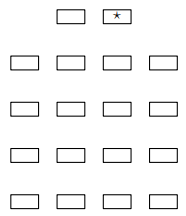
\includegraphics[scale=0.5]{desks.png}
\end{figure}
\item The 26 letters of the English alphabet are placed in a bag. Five of these letters are vowels and the rest are consonants. Mary draws one letter uniformly at random and writes it down. She doesn't put her letter back in the bag. Steph then draws a letter uniformly at random from the letters that remain in the bag. What is the probability that:
\begin{enumerate}
\item Mary's and Steph's letters are both vowels?
\item the two girls collectively have one vowel and one consonant?\vspace{1cm}
\end{enumerate}
\item (2011 State Sprint \#29) A bag contains red balls and white balls. If five balls are to be pulled from the bag one at a time with replacement, the probability of getting exactly three red balls is 32 times the probability of getting exactly one red ball. What percent of the balls originally in the bag are red?
\end{enumerate} 


% \newpage

% \section*{Repeated Elements}

% \begin{enumerate}
% \item If all the letters of the word $SYZYGY$\footnote{``In astronomy, a roughly straight-line configuration of three or more celestial bodies.''} are used, in how many different ways can the six letters be arranged in a six-letter string?\vspace{4cm}
% \item In how many different ways can the letters in the word $PEOPLE$ be scrambled, including the original spelling $PEOPLE$?\vspace{4cm}
% \item (2006 State Sprint Problem 28) Derek's phone number, 336-7624, has the property that the three-digit prefix, 336, equals the product of the last four digits, $7\times 6\times 2\times 4$. How many seven-digit phone numbers beginning with 336 have this property?
% \end{enumerate}


\newpage

\section*{Extensions}
\vspace{1cm}
\begin{enumerate}
\item \underline{\hspace{3in}} (2011 State Countdown)\vspace{1cm}
\item \underline{\hspace{3in}} [common fraction]\vspace{1cm}
\item \underline{\hspace{3in}}\vspace{1cm}
\item \underline{\hspace{3in}}\vspace{1cm}
\item \underline{\hspace{3in}} [common fraction]\vspace{1cm}
\item \begin{enumerate}
\item \underline{\hspace{2.7in}} [common fraction]\vspace{1cm}
\item \underline{\hspace{2.7in}} [common fraction]\vspace{1cm}
\end{enumerate}
\item \underline{\hspace{3in}} [common fraction] (2011 State Sprint \#27)
\end{enumerate}


\newpage

\section*{Extra Problems ($\star$)}

\begin{enumerate}
\item Let $A,B,C,D$ be integers and suppose
\begin{equation*}
x^4 + Ax^3 + Bx^2 + Cx + D = 0
\end{equation*}
when $x = 2^{1/4} + 2^{1/2}$. Compute $A + B + C + D$.\vspace{3cm}
\item For each positive integer $N$, let $P(N)$ be the probability that when a subset of $\{1, 2, \ldots, N\}$ is selected uniformly at random, the number of elements in the subset is a multiple of 4. For how many positive integers $N\leq 2025$ is it the case that $P(N) = 1/4$?\vspace{3cm}
\item In triangle $ABC$, points $E$ and $F$ are the midpoints of $\overline{AC}$ and $\overline{AB}$, respectively. Lines $\overline{BE}$ and $\overline{CF}$ intersect at $G$. If $\angle GBC = 60^{\circ}$ and $\angle GCB = 45^{\circ}$ and $BG = 4$, then what is $(BF)^2$? Express your answer in simplest radical form.\vspace{3cm}
\item How many (non-congruent) right triangles are there in which:
\begin{enumerate}
\item one of the leg lengths is 2025 and the other two side lengths are positive integers?
\item the hypotenuse has length 2025 and the two leg lengths are positive integers?
\end{enumerate}
\end{enumerate}


\end{document}